\documentclass[a4paper,francais,titlepage]{report}
\usepackage[utf8x]{inputenc}  
%% utf8x support des espaces insécables ' ' au lieu da la macro ~)

\usepackage[T1]{fontenc}
\usepackage[francais]{babel}
\usepackage{latexsym}
\usepackage{url}
\usepackage{graphicx}
\usepackage{enumerate}
\usepackage{lscape}   %% pour le mode paysage \begin{landscape}
\usepackage{hyperref}
\hypersetup{
    colorlinks,
    citecolor=black,
    filecolor=black,
    linkcolor=black,
    urlcolor=black
}

% continuité numérotation figures
\usepackage{chngcntr} 
\counterwithout{figure}{chapter}

% style général
\usepackage{fancyhdr}
\usepackage{vmargin}

\setmarginsrb{2.5cm}{2cm}{2.5cm}{1cm}{0.5cm}{1.5cm}{2cm}{2cm}
%1 est la marge gauche
%2 est la marge en haut
%3 est la marge droite
%4 est la marge en bas
%5 fixe la hauteur de l'entête
%6 fixe la distance entre l'entête et le texte
%7 fixe la hauteur du pied de page
%8 fixe la distance entre le texte et le pied de page

%%ressources
\graphicspath{{../ressources/}}

\begin{document}
\pagestyle{fancy}

%%%%%%%%% Première page: titre
\begin{titlepage}
 \begin{center}
	\vspace*{3.5cm}
	\Large \textbf{Gifts4YourFriends} \\
	\vspace{0.2cm}
	\small Rapport
	\vspace{2cm}

	\huge \textbf{Nuit de l'informatique} \\
	\vspace{0.3cm}
	\large {Défi Zenika}
	\vspace{1.5cm}
 \end{center}
 
 \begin{flushleft}
	\normalsize {\hspace{6cm}Responsables de l'événement: \\ 
				 \hspace{7.0cm} Blanc Xavier \\
				 \hspace{6.7cm} Bromberg David \\
				 \hspace{6.6cm} Fleury Emmanuel}
	\vspace{2cm}
 \end{flushleft}
 
   \begin{center}
   
\includegraphics[scale=0.3]{logo_bx1.jpg}
   	\vfill 
   	\vspace{2cm}
	\normalsize {Rage Against The Turing Machine\\}
	\vspace{1.5cm} 
	{\today}.
 \end{center}
\end{titlepage}
%%%%%%%% Fin première page

\section{Présentation de SCRUM}
SCRUM est une méthode agile de développement et permet au petites équipes de gérer un projet en permettant de rester souple et ouvert face aux changements des besoins du client. Cette méthode est composée d'une analyse complète (backlog) et est ensuite découpée en sprints qui durent généralement trois, quatre semaines. Cependant, pour tenir les deadlines du concours, nous avons fait des sprints de 4 heures. Chacun d'eux est composé de plusieurs tâches à implémenter puis tester.
\section{Répartition des tâches}
Compte tenu du nombre de défis que nous avons relevé, nous avons profité du grand nombre de personnes dans l'équipe et dispatcher l'effectif au différentes parties des défis. Six personnes s'occupaient de mettre en place le web service et la base de données correspondante. Trois personnes etaient responsables de l'interface Android. Trois autres de l'interface windows phone 7 et les trois dernières réalisaient le site avec google web toolkit.\\ Une personne par 'sous-equipe était désignée en tant que scrum-master suppléant. A chaque fin de sprint, un point était fait pour valider l'avancée des différentes tâches à exécuter et affecter les nouvelles.
Pour nous aider dans notre gestion de projet nous avons utilisé un tableau blanc et des post-it. Comme visible ci-dessous:\\
\begin{center}
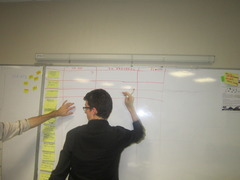
\includegraphics[scale=0.3]{backlog.jpeg}
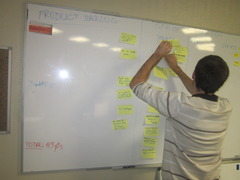
\includegraphics[scale=0.3]{backlog2.jpeg}
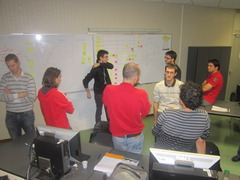
\includegraphics[scale=0.3]{brainstorming.jpeg}
\\
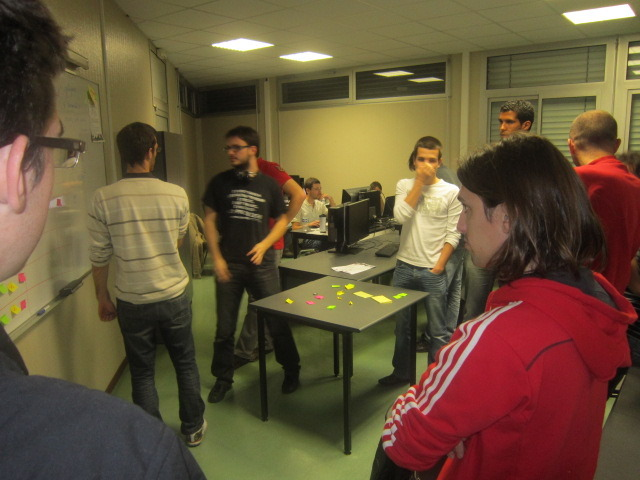
\includegraphics[scale=0.3]{brainstorming2.jpeg}\\
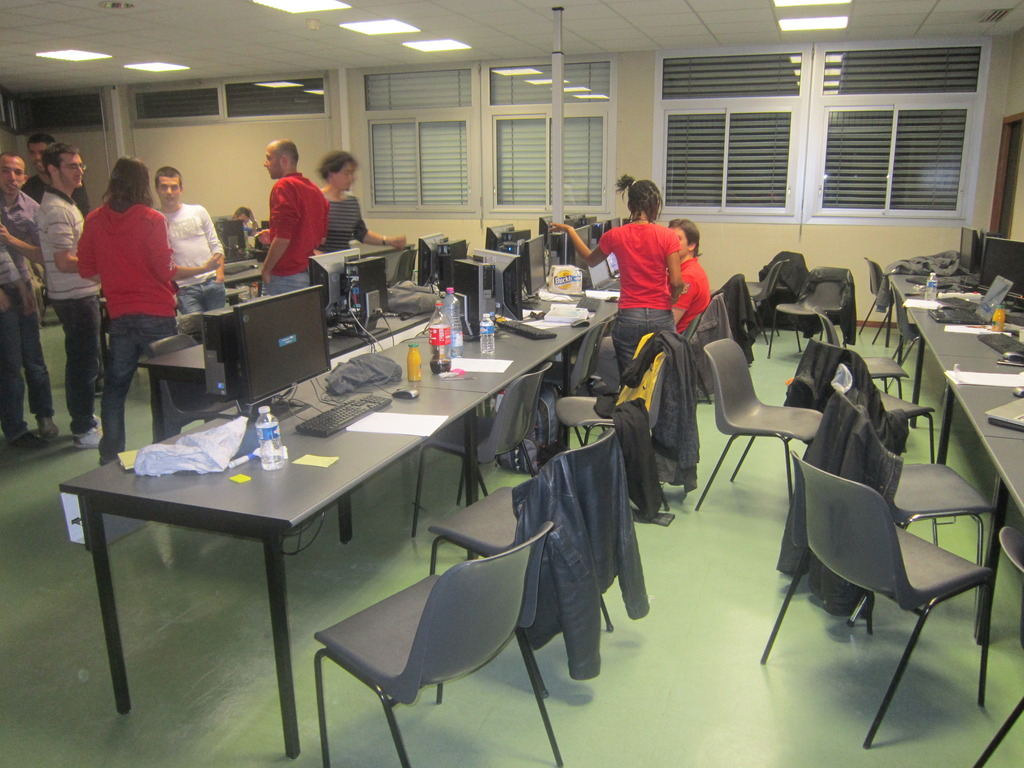
\includegraphics[scale=0.3]{brainstorming3.jpeg}
\\
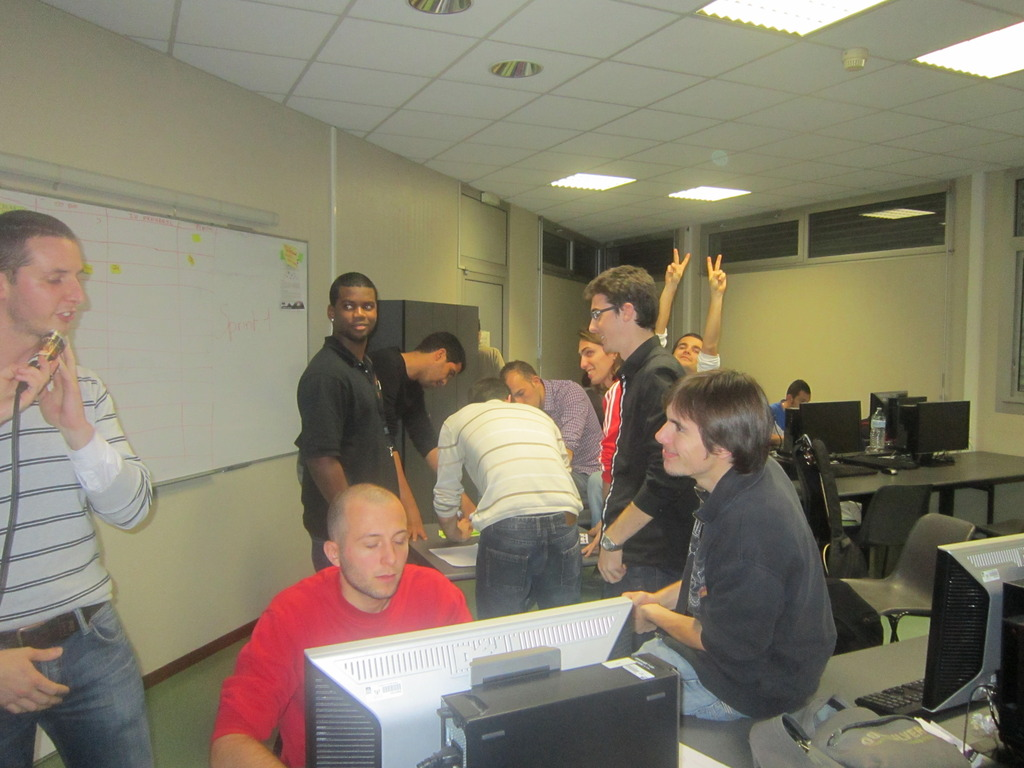
\includegraphics[scale=0.3]{brainstorming4.jpeg}
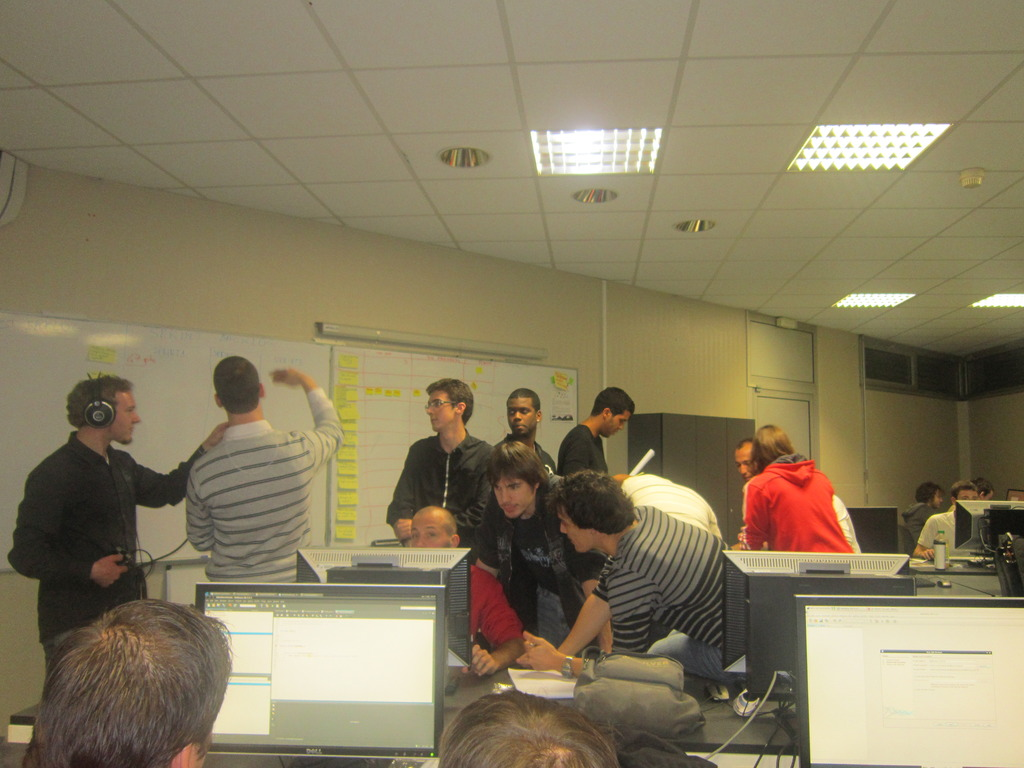
\includegraphics[scale=0.3]{brainstorming5.jpeg}
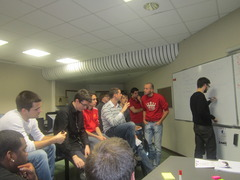
\includegraphics[scale=0.3]{brainstorming6.jpeg}
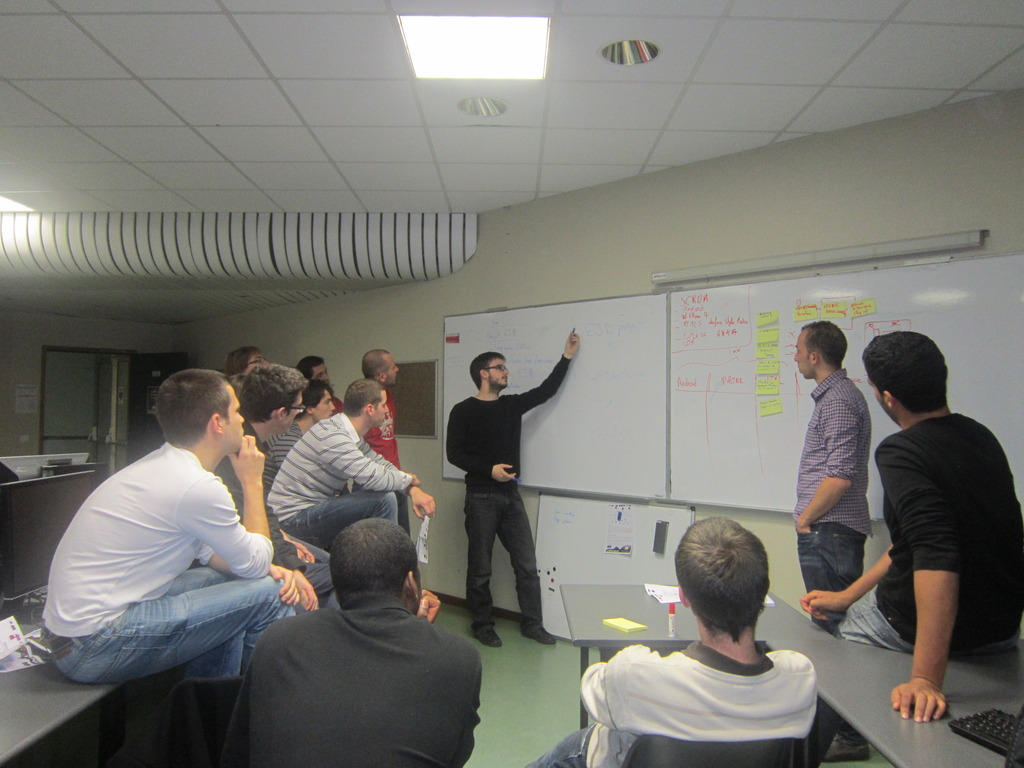
\includegraphics[scale=0.3]{brainstorming7.jpeg}
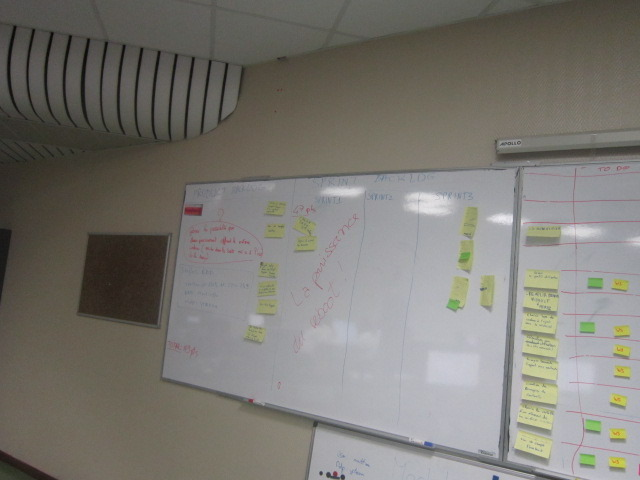
\includegraphics[scale=0.3]{tableau.jpeg}
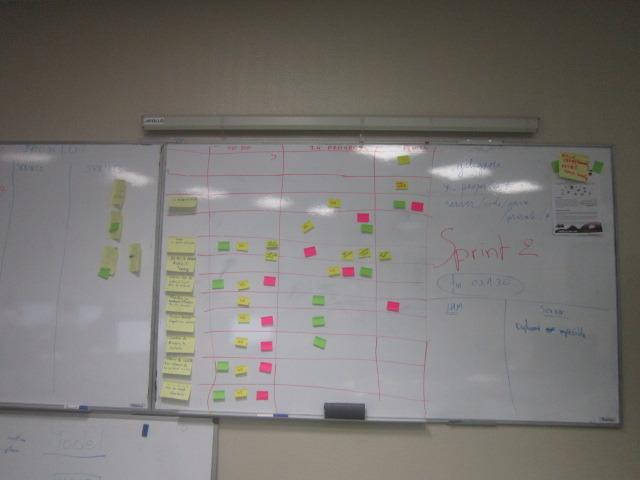
\includegraphics[scale=0.3]{tableau2.jpeg}
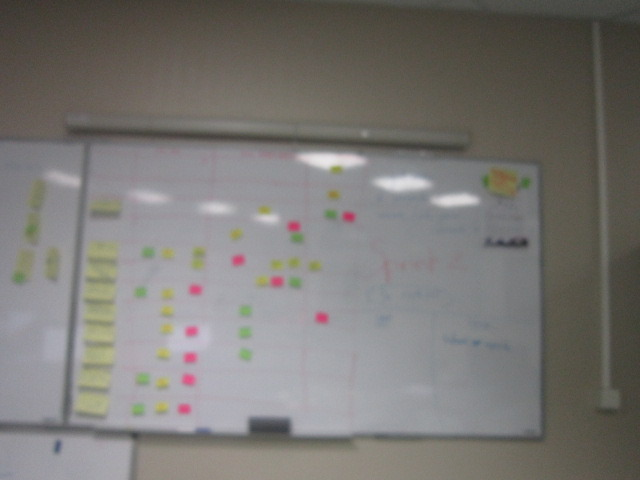
\includegraphics[scale=0.3]{tableau3.jpeg}
\end{center}
\newpage
\section{Bilan}
Nous pensons avoir bien mis en pratique la méthode SCRUM. Par ailleurs, dans le but de maximiser la communication et mettre du dynamisme durant cette nuit, nous avons créer un compte twitter auquel tout le groupe avait accès. Cependant, nous avons rencontré un certain nombre de problèmes.
Ces derniers partent des coupures intempestives au niveau du CREMI, qui nous ont obligé ne serait-ce que les deux premières fois, à recommencer les codes non enregistrées.
Puis, après des heures de configuration, nous avons appris que nous ne pouvions pas générer le .jar de notre projet Netbeans du fait de la sécurité au CREMI. 
Ainsi, aux environs de 1h du matin, nous avons dû changer d'IDE et passer sous Eclipse et passer à JBOSS en lieu et place de Glassfish sous Netbeans.

En résumé, il est beaucoup plus aisé de créer des web services sous Netbeans. Sous Eclipse, Il nous fallait des plug-ins, qui n'étaient pas installés sur les versions d'Eclipse mis à notre disposition. Voulant les installer sur nos machines personnelles, nous ne trouvions pas dans les "sites disponibles" pour l'installation de JBOSS WS notamment et son intégration dans le JBOSS pour la génération d'un web service.

La partie du serveur contient le modèle, les factories et permet de gérer la persistance de nos classes java POJO. Par contre, la communication avait les clients n'a pas pu être achevée.





\end{document}	